\documentclass[12pt, titlepage]{article}

\usepackage{booktabs}
\usepackage{float}
\usepackage{tabularx}
\usepackage{hyperref}
\usepackage{graphicx}
\hypersetup{
    colorlinks,
    citecolor=black,
    filecolor=black,
    linkcolor=red,
    urlcolor=blue
}
\usepackage[round]{natbib}
\usepackage{pdflscape}
\usepackage{longtable}
\usepackage{graphicx}

\input{../Comments}
%% Common Parts

\newcommand{\progname}{Software Engineering} % PUT YOUR PROGRAM NAME HERE
\newcommand{\authname}{Team \#2, Team Name
\\ Zihao Du 
\\ Matthew Miller
\\ Firas Elayan
\\ Abhiram Neelamraju
\\ Michael Kim} % AUTHOR NAMES                  

\usepackage{hyperref}
    \hypersetup{colorlinks=true, linkcolor=blue, citecolor=blue, filecolor=blue,
                urlcolor=blue, unicode=false}
    \urlstyle{same}
                                


\begin{document}

\title{Verification and Validation Report: \progname} 
\author{\authname}
\date{\today}
	
\maketitle

\pagenumbering{roman}

\section{Revision History}

\begin{tabularx}{\textwidth}{p{3cm}p{2cm}X}
\toprule {\bf Date} & {\bf Version} & {\bf Notes}\\
\midrule
Mar 4 & 1.0 & Add functional requirements evaluation\\
Mar 6 & 1.0 & Add non-functional requirements evaluation\\
Mar 6 & 1.0 & Load test, Usability test, unit test results\\
Mar 6 & 1.0 & Add Automated test, non-dynamic test result and changes due to testing\\
Apr 2 & 1.1 & Resolve team 11 feedback\\
Apr 3 & 1.1 & Resolve TA feedback about functional and non functional tests\\
\bottomrule
\end{tabularx}

~\newpage

\section{Symbols, Abbreviations and Acronyms}

\renewcommand{\arraystretch}{1.2}
\begin{tabular}{l l} 
  \toprule		
  \textbf{symbol} & \textbf{description}\\
  \midrule 
  APK & Android Application Package\\
  \midrule 
  AR & Augmented reality\\
  \midrule 
  Azure & A cloud computing platform run by Microsoft\\
  \midrule 
  CI & Continuous integration\\
  \midrule 
  JHE & John Hodgins Engineering Building\\
  \midrule 
  JMeter & Load testing tool for analyzing and measuring the performance\\
  \midrule 
  NUnit & An open-source unit testing framework for the .NET Framework and Mono\\
  \midrule 
  OpenCover & An open source code coverage tool\\
  \midrule 
  SRS & Software Requirements Specification\\
  \midrule
  TA & Teaching Assistant\\
  \midrule 
  UI & User Interface\\
  \midrule 
  UTF & Unity Test Framework\\
  \midrule 
  VnV & Verification and Validation\\
  \midrule 
  XML & Extensible Markup Language\\
  \bottomrule
\end{tabular}\\

\newpage

\tableofcontents

\listoftables %if appropriate

\listoffigures %if appropriate

\newpage

\pagenumbering{arabic}

This document describes the test results of the verification and validation (VnV) plan for CampusConnections. The VnV plan was continuously updated as the project evolved. The following document records the results of the current version of the VnV plan. It provides results of functional and non-functional requirements tests, unit tests, changes that will be implemented in the system as a result of the tests, and various traceability tables.


\section{Functional Requirements Evaluation}
The following section outlines the results of functional requirements testing. The process and test performed follow the \href{https://github.com/beatlepie/4G06CapstoneProjectTeam2/blob/main/docs/VnVPlan/VnVPlan.pdf}{VnV Plan}. To summarize, all the tests are tested manually and passed, indicating that all the functional requirements in the Software Requirements Specification (\href{https://github.com/beatlepie/4G06CapstoneProjectTeam2/blob/main/docs/SRS/SRS.pdf}{SRS}) document are covered.

\subsection{Pre-Registration Settings}
This section covers all tests related to functional requirements about pre-registration settings.
\begin{enumerate}
\item \textbf{FRT-PR1}

\textbf{Name:} Agree To Consent Form

\textbf{Initial State:} The user does not have an account, and they starts to register an account. A consent form appears asking for access to the device and permission to collect user data

\textbf{Input:} The user agrees to all the terms and conditions and clicks `Agree' and continues to complete the registration process
					
\textbf{Expected Output:} A notification shows the registration succeeds and the user is redirected to the login screen

\textbf{Actual Output:} A notification shows the registration succeeds and the user is redirected to the login screen

\textbf{Results:} Pass

\item \textbf{FRT-PR2}

\textbf{Name:} Disagree To Consent Form

\textbf{Initial State:} The user does not have an account, and they starts to register an account. A consent form appears asking for access to the device and permission to collect user data
					
\textbf{Input:} The user rejects the terms and conditions and clicks `Disagree' and continues to complete the registration process
					
\textbf{Expected Output:} The registration fails and a warning will show up notifying the user that they cannot create an account unless they agree to the consent form

\textbf{Actual Output:} The registration fails and a warning will show up notifying the user that they cannot create an account unless they agree to the consent form

\textbf{Results:} Pass
\end{enumerate}
\subsection{User Account}
This section covers all tests related to functional requirements about the account and user profile.
\begin{enumerate}
\item \textbf{FRT-UA1}

\textbf{Name:} Successful Account Creation

\textbf{Initial State:} The user does not have an account and is not logged in to the application

\textbf{Input:} All information needed to create an account:
\begin{itemize}
\item Email: testUA1@gmail.com
\item password: FRT-UA1
\item nickname: UA1
\end{itemize}
					
\textbf{Expected Output:} An Account with corresponding information is created in the database with the account initialized to INITIAL\_USER\_STATE

\textbf{Actual Output:} An Account is created in the database with the following attributes and other attributes are initialized to INITIAL\_USER\_STATE:
\begin{itemize}
\item Email: testUA1@gmail.com
\item password: FRT-UA1
\item nickname: UA1
\end{itemize}

\textbf{Results:} Pass

\item \textbf{FRT-UA2}

\textbf{Name:} Unsuccessful Account Creation With Existing Email

\textbf{Initial State:} The user does not have an account and is not logged in to the application

\textbf{Input:} All information needed to create an account:
\begin{itemize}
\item Email: qtest@gmail.com (this is an existing test account)
\item password: FRT-UA1
\item nickname: UA1
\end{itemize}
					
\textbf{Expected Output:} Account creation fails with a warning telling the user the email has already been used

\textbf{Actual Output:} Account creation fails with a warning telling the user the email has already been used

\textbf{Results:} Pass

\item \textbf{FRT-UA3}

\textbf{Name:} Successful Account Login

\textbf{Initial State:} The user has an account and is not logged in to the application

\textbf{Input:} All information needed to login:
\begin{itemize}
\item Email: FRT-UA3@test.com (this account exists in the system already)
\item password: FRT-UA3
\end{itemize}
					
\textbf{Expected Output:} User successfully logs into the application and goes to the menu page

\textbf{Actual Output:} User successfully logs into the application and goes to the menu page

\textbf{Results:} Pass

\item \textbf{FRT-UA4}

\textbf{Name:} Unsuccessful Account Login With Wrong Password

\textbf{Initial State:} The user has an account and is not logged in to the application

\textbf{Input:} All information needed to login:
\begin{itemize}
\item Email: FRT-UA3@test.com (this account exists in the system already)
\item password: FRT321 (wrong password)
\end{itemize}
					
\textbf{Expected Output:} Login fails with a warning telling the user the password is wrong

\textbf{Actual Output:} Login fails with a warning telling the user the password is wrong

\textbf{Results:} Pass

\item \textbf{FRT-UA5}

\textbf{Name:} Account Deletion

\textbf{Initial State:} The user has an account and is logged into the application
\begin{itemize}
\item Email: FRT-UA5@gmail.com (this is an existing test account)
\item password: FRT-UA5
\item nickname: UA5
\end{itemize}

\textbf{Input:} User clicks on the delete account button on the profile page and confirms the deletion
					
\textbf{Expected Output:} The user is redirected to the login page and the account cannot be logged in any more

\textbf{Actual Output:} The user is redirected to the login page and the account FRT-UA5@gmail.com cannot be logged in any more

\textbf{Results:} Pass

\item \textbf{FRT-UA6}

\textbf{Name:} Reset Password

\textbf{Initial State:} The user has an account:
\begin{itemize}
\item Email: campusconnections@gmail.com (this is an existing test account)
\item password: qtesting
\end{itemize}

\textbf{Input:} Email address and new password
\begin{itemize}
\item new password: QTesting
\end{itemize}
					
\textbf{Expected Output:} Password is successfully reset

\textbf{Actual Output:} Password is successfully reset to be QTesting

\textbf{Results:} Pass

\item \textbf{FRT-UA7}

\textbf{Name:} Avatar Creation and Modification

\textbf{Initial State:} The user has an account with DEFAULT\_AVATAR

\textbf{Input:} URI represents the new avatar:
\begin{itemize}
\item URI: https://upload.wikimedia.org/wikipedia/commons/2/2f/Google\_2015\_logo.svg
\end{itemize}
					
\textbf{Expected Output:} The user changes the avatar to a Google logo

\textbf{Actual Output:} The user changes the avatar to a Google logo

\textbf{Results:} Pass

\item \textbf{FRT-UA8}

\textbf{Name:} Email Verification

\textbf{Initial State:} The user has an account whose email has not been verified yet
\begin{itemize}
\item Email: fuz15@mcmaster.ca (this is an existing test account)
\item password: password
\end{itemize}

\textbf{Input:} User clicks on `Verify Email` button on user profile page and follows instructions on the email sent from the system
					
\textbf{Expected Output:} That email above is verified as a valid email address

\textbf{Actual Output:} fuz15@mcmaster.ca is verified as a valid email address in the system

\textbf{Results:} Pass

\item \textbf{FRT-UA9}

\textbf{Name:} Edit Profile

\textbf{Initial State:} The user has an account 
\begin{itemize}
\item Email: qtest@gmail.com (this is an existing test account)
\item password: qtesting
\item program: Software Engineering
\end{itemize}

\textbf{Input:} New Profile:
\begin{itemize}
\item newProgram: Computer Science
\item newLevel: 4
\end{itemize}
					
\textbf{Expected Output:} The program and level are updated

\textbf{Actual Output:} The program and level are updated to be Computer Science and 4

\textbf{Results:} Pass
\end{enumerate}
\subsection{Social Networking System}
This section covers all tests related to functional requirements about interactions between friends.
\begin{enumerate}
\item \textbf{FRT-SN1}

\textbf{Name:} Successful Friend Request

\textbf{Initial State:} The user is logged in with the following account:
\begin{itemize}
\item Femail: FRT-SN1@test.com
\item password: testing
\end{itemize}

\textbf{Input:} A valid email to send the request:
\begin{itemize}
\item Temail: FRT-SN1-F@test.com
\end{itemize}
					
\textbf{Expected Output:} A Friend request is sent to the target user and available to be accepted or rejected by the target user in the request list

\textbf{Actual Output:} A Friend request is sent to the target user and available to be accepted or rejected by the target user in the request list

\textbf{Results:} Pass

\item \textbf{FRT-SN2}

\textbf{Name:} Friend Request Acceptance

\textbf{Initial State:} A friend request was sent from an account (Femail) to the target account (Temail):
\begin{itemize}
\item Femail: FRT-SN1@test.com
\item Temail: FRT-SN1-F@test.com
\end{itemize}

\textbf{Input:} The request is accepted
					
\textbf{Expected Output:} Two users are added to each other's friend lists

\textbf{Actual Output:} Two users are added to each other's friend lists

\textbf{Results:} Pass

\item \textbf{FRT-SN3}

\textbf{Name:} Successful Friend Rejection

\textbf{Initial State:} A friend request was sent from an account (Femail) to the target account (Temail):
\begin{itemize}
\item Femail: FRT-SN1@test.com
\item Temail: FRT-SN1-F@test.com
\end{itemize}

\textbf{Input:} The request is rejected
					
\textbf{Expected Output:} The request is declined and no friend is added for both accounts

\textbf{Actual Output:} The request is declined and no friend is added for both accounts

\textbf{Results:} Pass

\item \textbf{FRT-SN4}

\textbf{Name:} Friend Deletion

\textbf{Initial State:} A friend (Femail) exist in the friend list of the test account (Temail):
\begin{itemize}
\item Temail: FRT-SN4@test.com
\item Femail: FRT-SN4-F@test.com
\end{itemize}

\textbf{Input:} User deletes the chosen friend
					
\textbf{Expected Output:} The corresponding friend is deleted from the list

\textbf{Actual Output:} The corresponding friend FRT-SN4-F@test.com is deleted from the friend list

\textbf{Results:} Pass

\item \textbf{FRT-SN5}

\textbf{Name:} Friend Messaging

\textbf{Initial State:} A friend (Femail) exist in the friend list of the test account (Temail):
\begin{itemize}
\item Temail: FRT-SN5@test.com
\item Femail: FRT-SN5-F@test.com
\end{itemize}

\textbf{Input:} Message: `Hello World'
					
\textbf{Expected Output:} The corresponding message is sent to the friend

\textbf{Actual Output:} The corresponding message is sent to the friend

\textbf{Results:} Pass

\item \textbf{FRT-SN6}

\textbf{Name:} Friend Sharing Event

\textbf{Initial State:} A friend (Femail) exist in the friend list of the test account (Temail):
\begin{itemize}
\item Temail: FRT-SN6@test.com
\item Femail: FRT-SN6-F@test.com
\end{itemize}

\textbf{Input:} Message that contains event name and follows some specific pattern:
Hey, check this event: \textunderscore E\textunderscore[EXPO]
					
\textbf{Expected Output:} User is redirected to the event page with that event once they click on the message

\textbf{Actual Output:} User is redirected to the event page with a filter on event name: EXPO

\textbf{Results:} Pass

\item \textbf{FRT-SN7}

\textbf{Name:} Friend Sharing Lecture

\textbf{Initial State:} A friend (Femail) exist in the friend list of the test account (Temail):
\begin{itemize}
\item Temail: FRT-SN7@test.com
\item Femail: FRT-SN7-F@test.com
\end{itemize}

\textbf{Input:} Message that contains lecture code and follows some specific pattern:
`Hey, are you in this lecture: \textunderscore L\textunderscore[SFRWENG 4G06]'
					
\textbf{Expected Output:} User is redirected to the lecture page with that lecture once they click on the message

\textbf{Actual Output:} User is redirected to the lecture page with a filter on lecture code: SFRWENG 4G06

\textbf{Results:} Pass
\end{enumerate}
\subsection{Lectures and Events}
This section covers all tests related to functional requirements about lectures and events and how users can interact with them.
\begin{enumerate}
\item \textbf{FRT-LE1}

\textbf{Name:} Save Event

\textbf{Initial State:} A sample event:
\begin{itemize}
\item Name: EXPO
\end{itemize}

\textbf{Input:} On the event page, user clicks on the save button on the pop-up window with details of the sample event
					
\textbf{Expected Output:} The event is saved to the user's event list

\textbf{Actual Output:} The event EXPO is saved to the user's event list

\textbf{Results:} Pass

\item \textbf{FRT-LE2}

\textbf{Name:} Unsave Event

\textbf{Initial State:} A sample event that is already been saved:
\begin{itemize}
\item Name: EXPO
\end{itemize}

\textbf{Input:} On the event page, user clicks on the unsave button on the pop-up window with details of the sample event
					
\textbf{Expected Output:} The event is removed from the user's event list

\textbf{Actual Output:} The event EXPO is removed from the user's event list

\textbf{Results:} Pass

\item \textbf{FRT-LE3}

\textbf{Name:} Save Lecture

\textbf{Initial State:} A sample lecture:
\begin{itemize}
\item Code: SFWRENG 4G06
\end{itemize}

\textbf{Input:} On the lecture page, user clicks on the save button on the pop-up window with details of the sample lecture
					
\textbf{Expected Output:} The lecture is saved to the user's lecture list

\textbf{Actual Output:} The lecture SFWRENG 4G06 is saved to the user's lecture list

\textbf{Results:} Pass

\item \textbf{FRT-LE4}

\textbf{Name:} Unsave Lecture

\textbf{Initial State:} A sample lecture that is already been saved:
\begin{itemize}
\item Code: SFWRENG 4G06
\end{itemize}

\textbf{Input:} On the lecture page, user clicks on the unsave button on the pop-up window with details of the sample lecture
					
\textbf{Expected Output:} The lecture is removed from the user's lecture list

\textbf{Actual Output:} The lecture SFWRENG 4G06 is removed from the user's lecture list

\textbf{Results:} Pass

\item \textbf{FRT-LE5}

\textbf{Name:} Administrator Add Event

\textbf{Initial State:} User is logged in as an administrator
\begin{itemize}
\item email: campusconnections@gmail.com
\item password: testing
\end{itemize}

\textbf{Input:} Sample event:
\begin{itemize}
\item name: Test event
\item description: Sample event for system test
\item time: 0
\item duration: 0
\item location: Online
\item isPublic: true
\item organizer: Team 2
\end{itemize}
					
\textbf{Expcted Output:} The event is added to the event list

\textbf{Actual Output:} The event Test event is added to the event list

\textbf{Results:} Pass

\item \textbf{FRT-LE6}

\textbf{Name:} Administrator Add Event With Existing Name

\textbf{Initial State:} User is logged in as an administrator
\begin{itemize}
\item email: campusconnections@gmail.com
\item password: testing
\end{itemize}

Sample event exists:
\begin{itemize}
\item name: Test event
\item description: Sample event for system test
\item time: 0
\item duration: 0
\item location: Online
\item isPublic: true
\item organizer: Team 2
\end{itemize}

\textbf{Input:} New sample event:
\begin{itemize}
\item name: Test event
\item description: New sample event
\item time: 100
\item duration: 30
\item location: TBD
\item isPublic: false
\item organizer: TBD
\end{itemize}
					
\textbf{Expcted Output:} The sample event is update to be the same as the input event

\textbf{Actual Output:} The sample event is update to be the same as the input event

\textbf{Results:} Pass

\item \textbf{FRT-LE7}

\textbf{Name:} Administrator Edit Event

\textbf{Initial State:} User is logged in as an administrator
\begin{itemize}
\item email: campusconnections@gmail.com
\item password: testing
\end{itemize}

\textbf{Input:} Sample event name and new location:
\begin{itemize}
\item name: Test event
\item location: ITB AB102
\end{itemize}
					
\textbf{Expected Output:} The test event location is updated to the new one

\textbf{Actual Output:} The test event location is updated to ITB AB102

\textbf{Results:} Pass

\item \textbf{FRT-LE8}

\textbf{Name:} Administrator Delete Event

\textbf{Initial State:} User is logged in as an administrator
\begin{itemize}
\item email: campusconnections@gmail.com
\item password: testing
\end{itemize}

\textbf{Input:} Sample event (already in the system) name:
\begin{itemize}
\item name: Test event
\end{itemize}
					
\textbf{Expected Output:} The event is deleted and disappears from the list

\textbf{Actual Output:} The Test event is deleted and disappears from the list

\textbf{Results:} Pass

\item \textbf{FRT-LE9}

\textbf{Name:} Administrator Add Lecture

\textbf{Initial State:} User is logged in as an administrator
\begin{itemize}
\item email: campusconnections@gmail.com
\item password: testing
\end{itemize}

\textbf{Input:} Sample lecture:
\begin{itemize}
\item code: TEST 1T03
\item name: Test lecture
\item time: 12:00 - 13:00, Mon
\item location: Online
\item instructor: NA
\end{itemize}
					
\textbf{Expected Output:} The lecture is added to the lecture list

\textbf{Actual Output:} The lecture TEST 1T03 is added to the lecture list

\textbf{Results:} Pass

\item \textbf{FRT-LE10}

\textbf{Name:} Administrator Add Lecture With Existing Code

\textbf{Initial State:} User is logged in as an administrator
\begin{itemize}
\item email: campusconnections@gmail.com
\item password: testing
\end{itemize}

A sample lecture exists:
\begin{itemize}
\item code: TEST 1T03
\item name: Test lecture
\item time: 12:00 - 13:00, Mon
\item location: Online
\item instructor: NA
\end{itemize}

\textbf{Input:} New sample lecture:
\begin{itemize}
\item code: TEST 1T03
\item name: New test lecture
\item time: 12:00 - 13:00, Wed
\item location: TBD
\item instructor: TBD
\end{itemize}
					
\textbf{Expected Output:} The sample lecture is update to be the same as the input lecture

\textbf{Actual Output:} The sample lecture is update to be the same as the input lecture

\textbf{Results:} Pass

\item \textbf{FRT-LE9}

\textbf{Name:} Administrator Edit Lecture

\textbf{Initial State:} User is logged in as an administrator
\begin{itemize}
\item email: campusconnections@gmail.com
\item password: testing
\end{itemize}

\textbf{Input:} Sample lecture name and new location:
\begin{itemize}
\item code: TEST 1T03
\item location: ITB AB102
\end{itemize}
					
\textbf{Expected Output:} The test lecture location is updated to the new one

\textbf{Actual Output:} The test lecture location is updated to ITB AB102

\textbf{Results:} Pass

\item \textbf{FRT-LE10}

\textbf{Name:} Administrator Delete Lecture

\textbf{Initial State:} User is logged in as an administrator
\begin{itemize}
\item email: campusconnections@gmail.com
\item password: testing
\end{itemize}

\textbf{Input:} Sample lecture (already in the system) name:
\begin{itemize}
\item code: TEST 1T03
\end{itemize}
					
\textbf{Expected Output:} The lecture is deleted and disappears from the list

\textbf{Actual Output:} The test lecture is deleted and disappears from the list

\textbf{Results:} Pass

\item \textbf{FRT-LE11}

\textbf{Name:} Event Information

\textbf{Initial State:} A sample event exists:
\begin{itemize}
\item name: EXPO
\end{itemize}

\textbf{Input:} User clicks on the sample event
					
\textbf{Expected Output:} All event information is shown in a pop-up window

\textbf{Actual Output:} All event information is shown in a pop-up window:
\begin{itemize}
\item name
\item description
\item location
\item time
\item duration
\item organizer
\item isPublic
\end{itemize}

\textbf{Results:} Pass

\item \textbf{FRT-LE12}

\textbf{Name:} Lecture Information

\textbf{Initial State:} A sample lecture exists:
\begin{itemize}
\item code: SFWRENG 4G06
\end{itemize}

\textbf{Input:} User clicks on the sample lecture
					
\textbf{Expected Output:} All lecture information is shown in a pop-up window

\textbf{Actual Output:} All lecture information is shown in a pop-up window:
\begin{itemize}
\item code
\item name
\item instructor
\item time
\item location
\end{itemize}

\textbf{Results:} Pass

\item \textbf{FRT-LE13}

\textbf{Name:} Lecture Filter by Code

\textbf{Initial State:} Some software engineering lectures exist in the system with the following course codes (other attributes of lecture do not affect the test and can be empty):
\begin{itemize}
\item SFWRENG 4G06
\item SFWRENG 4E03
\item COMPSCI 4TB3
\end{itemize}

\textbf{Input:} Filter:
\begin{itemize}
\item FilterString: SFWRENG
\end{itemize}
					
\textbf{Expected Output:} All lectures which do not contain the FilterString in the code are removed from the list (COMPSCI 4TB3 in this case)

\textbf{Actual Output:} All lectures which do not contain the SFWRENG in the code are removed from the list (COMPSCI 4TB3 in this case)

\textbf{Results:} Pass

\item \textbf{FRT-LE14}

\textbf{Name:} Event Filter by Name

\textbf{Initial State:} Some events exist in the system with following names (other attributes of event do not affect the test and can be empty):
\begin{itemize}
\item Job Fair: March 4
\item Job Fair: March 10
\item Rev 0 Demo
\end{itemize}

\textbf{Input:} Filter:
\begin{itemize}
\item FilterString: Job Fair
\end{itemize}
					
\textbf{Expected Output:} All events which do not contain the FilterString in the name are removed from the list (Rev 0 Demo in this case)

\textbf{Actual Output:} All events which do not contain the Job Fair in the name are removed from the list (Rev 0 Demo in this case)

\textbf{Results:} Pass
\end{enumerate}
\subsection{AR Camera}
This section covers all tests related to functional requirements about AR camera.
\begin{enumerate}
\item \textbf{FRT-AR1}

\textbf{Name:} Successful Building Recognition

\textbf{Initial State:} User is at the front door of JHE

\textbf{Input:} Clear camera view
					
\textbf{Expected Output:} The building (JHE) is recognized with its name and description shown as an AR object

\textbf{Actual Output:} The building (JHE) is recognized with its name and description shown as an AR object

\textbf{Results:} Pass

\item \textbf{FRT-AR2}

\textbf{Name:} Unsuccessful Building Recognition

\textbf{Initial State:} User is out of campus

\textbf{Input:} Clear camera view
					
\textbf{Expected Output:} No AR objects are shown

\textbf{Actual Output:} No AR objects are shown

\textbf{Results:} Pass

\item \textbf{FRT-AR3}

\textbf{Name:} Building Lectures/Events

\textbf{Initial State:} User is in JHE lobby

\textbf{Input:} Clear camera view
					
\textbf{Expected Output:} Event and lecture information separated by room number at the corresponding locations of the building

\textbf{Actual Output:} Event and lecture information separated by room number at the corresponding locations of the building

\textbf{Results:} Pass
\end{enumerate}
\subsection{Map and Location}
This section covers all tests related to functional requirements about the map and location tracking in the system.
\begin{enumerate}
\item \textbf{FRT-MAP1}

\textbf{Name:} User Location

\textbf{Initial State:} User allows the user to use their real-time location

\textbf{Input:} User enters the map page
					
\textbf{Expected Output:} A model representing the user shows up on the map and moves correspondingly when the user moves

\textbf{Actual Output:} A model representing the user shows up on the map and moves correspondingly when the user moves

\textbf{Results:} Pass

\item \textbf{FRT-MAP2}

\textbf{Name:} Friend Locations

\textbf{Initial State:} User has some friends who are willing to share locations:
\begin{itemize}
\item email1: MAP2-1@test.com
\item email2: MAP2-2@test.com
\end{itemize}

\textbf{Input:} User enters the map page
					
\textbf{Expected Output:} Additional models representing friends show up on the map and move correspondingly when friends move

\textbf{Actual Output:} Additional models representing friends show up on the map and move correspondingly when friends move

\textbf{Results:} Pass
\end{enumerate}

\section{Nonfunctional Requirements Evaluation}
The following section outlines the results of non-functional requirements testing. The process and test performed follow the \href{https://github.com/beatlepie/4G06CapstoneProjectTeam2/blob/main/docs/VnVPlan/VnVPlan.pdf}{VnV Plan}. Most of the tests are tested manually while some of them are tested in another way, for instance, load testing is tested with JMeter while some UI requirements are tested by conducting a survey, etc. \textcolor{red}{Some of the tests fail because their related requirements are removed due to the change of the project's scope, these tests will be marked in red.} In general, most of the tests in the plan succeed, indicating that non-functional requirements in the Software Requirements Specification (SRS) document are covered.
\subsection{Look and feel}
This section corresponds to the Look and feel tests in VnV Plan and Look and Feel requirements in SRS.
\begin{enumerate}
\item \textbf{NFRT-LF1}

\textbf{Name:} Survey for feedback on application layout

\textbf{Initial State:} Survey taker is given an account:
\begin{itemize}
\item email: mtest@gmail.com
\item password: mtesting
\end{itemize}

\textbf{Input:} Usability Survey in section \ref{survey}

\textbf{Expected Output:} Tasks are completed successfully and ``Immediate Visual Response when Clicking'' and ``Appealing Colour Scheme'' questions get average scores that are great than MIN\_SCORE

\textbf{Actual Output:} Tasks are completed successfully and ``Immediate Visual Response when Clicking'' and ``Appealing Colour Scheme'' questions get average scores of 3.8 and 4.8 respectively

\textbf{Result:} Pass

\item \textbf{NFRT-LF2}

\textbf{Name:} Visual inspection with different screen sizes

\textbf{Input/Condition:} User opens the application on the phone with all different screen sizes in the SCREEN\_VIEWPORTS list

\textbf{Expected Output:} For all different pages all visual elements on the screen are within the borders of the screen for all screens in the SCREEN\_VIEWPORTS list

\textbf{Actual Output:} All elements are within the borders of the screen without overlapping for all screen sizes in the SCREEN\_VIEWPORTS list

\textbf{Result:} Pass

\item \textbf{NFRT-LF3}

\textbf{Name:} Visual inspection of color scheme

\textbf{Initial State:} NA
					
\textbf{Input:} User opens the application on the phone

\textbf{Expected Output:} For all different pages the colour scheme is the same

\textbf{Actual Output:} For all different pages the colour of elements and texts is always maroon, gold, black and white

\textbf{Result:} Pass
\end{enumerate}
\subsection{Usability and Humanity}
This section corresponds to the Usability and Humanity tests in VnV Plan and Usability and Humanity requirements in SRS.
\begin{enumerate}
\item \textbf{NFRT-UH1}

\textbf{Name:} Survey for feedback on understandability and easy of use

\textbf{Initial State:} Survey taker is given an account:
\begin{itemize}
\item email: mtest@gmail.com
\item password: mtesting
\end{itemize}

\textbf{Input:} Usability Survey in section \ref{survey}

\textbf{Expected Output:} Tasks are completed successfully and ``No Technical or Software-Specific Language'' question gets an average score that is great than MIN\_SCORE

\textbf{Actual Output:} Tasks are completed successfully and ``No Technical or Software-Specific Language'' question gets an average score of 4

\textbf{Result:} Pass

\item \textbf{NFRT-UH2}

\textbf{Name:} Walkthrough of user guide

\textbf{Input:} GitHub web page (see details in section \ref{static})
					
\textbf{Expected Output:} The participants can see the main features are explained in the GitHub repo

\textbf{Actual Output:} The participants can see the main features are explained in the GitHub repo

\textbf{Result:} Pass

\item \textbf{NFRT-UH3}

\textbf{Name:} Visual inspection of color contrast

\textbf{Initial State:} NA
					
\textbf{Input:} User opens the application checks the color contrast statically

\textbf{Expected Output:} The color contrast is greater than 4.5:1,  the Web Content Accessibility Guidelines' AA standards for accessibility

\textbf{Actual Output:} The color contrasts are listed following:
\begin{itemize}
\item Maroon - White: 10.94:1
\item White - Black: 21:1
\item Gold - Black: 14.97:1
\item Maroon - Gold: 7.8:1
\end{itemize}

\textbf{Result:} Pass
\end{enumerate}
\subsection{Performance}
This section corresponds to the Performance tests in VnV Plan and Performance requirements in SRS.
\begin{enumerate}
\item \textbf{NFRT-P1}

\textbf{Name:} AR camera recognition

\textbf{Initial State:} The user is near or in a target building (JHE)
					
\textbf{Input:} User turns on AR camera
					
\textbf{Expected Output:} Corresponding AR objects appears within RECOGNITION\_TIME

\textbf{Actual Output:} Corresponding AR objects appears within 1 second

\textbf{Result:} Pass

\item \textbf{NFRT-P2}

\textbf{Name:} Real-time location update

\textbf{Initial State:} User allows the application to use device location
					
\textbf{Input:} User turns on the map and walks around on campus
					
\textbf{Expected Output:} The user model on the map is updated within  LOCATION\_UPDATE\_TIME when the user is moving

\textbf{Actual Output:} The user model is updated within 0.5 second if the user is outdoor, and indoor location update time is around 5 second (and sometimes not very accurate)

\textbf{Result:} Pass

\item \textbf{NFRT-P3}

\textbf{Name:} Code Walkthrough For User Personal Data

\textbf{Input:} Source code (see details in section \ref{static})

\textbf{Expected Output:} Successfully convinced the participants the following:
\begin{itemize}
  \item User's personal information does not appear in the database if the user did not grant permission
\end{itemize}

\textbf{Actual Output:} Successfully convinced the participants that the user personal information is collected under permission only

\textbf{Result:} Pass

\item \textbf{NFRT-P4}

\textbf{Name:} Code Walkthrough For Data Transmission Encryption

\textbf{Input:} Source code (see details in section \ref{static})

\textbf{Expected Output:} Successfully convinced the participants the following:
\begin{itemize}
  \item The product only transmits encrypted data from server to user
\end{itemize}

\textbf{Actual Output:} Successfully convinced the participants that the data send from/to the server are encrypted

\textbf{Result:} Pass

\item \textbf{NFRT-P5}

\textbf{Name:} Warning when starting AR camera

\textbf{Initial State:} User allows the application to use camera
					
\textbf{Input:} User turns on the AR camera
					
\textbf{Expected Output:} A warning telling the user to be aware of their surroundings is displayed upon start-up of the camera

\textbf{Actual Output:} A warning telling the user to be aware of their surroundings is displayed upon start-up of the camera

\textbf{Result:} Pass

\item \textbf{NFRT-P6}

\textbf{Name:} Leaving campus warning

\textbf{Initial State:} User opens the map
					
\textbf{Input:} User moves out of the campus
					
\textbf{Expected Output:} A warning message is displayed telling the user that the map is not available out of campus

\textbf{Actual Output:} A warning message is displayed telling the user that the map is not available out of campus and the user is redirected to the menu page once the warning message is closed

\textbf{Result:} Pass

\item \textbf{NFRT-P7}

\textbf{Name:} Special character warning

\textbf{Initial State:} User starts to register
					
\textbf{Input:} User enters nickname with some special character: `; DELETE *'
					
\textbf{Expected Output:} A warning message is displayed telling the user that the special characters are not allowed and stops the user from registering

\textbf{Actual Output:} A warning message is displayed telling the user that the special characters are not allowed and stops the user from registering

\textbf{Result:} Pass

\item \textbf{NFRT-P8}

\textbf{Name:} Email format warning

\textbf{Initial State:} User starts to register
					
\textbf{Input:} User enters a not email string in the email field:
`SELECT * FROM TABLE'
					
\textbf{Expected Output:} A warning message is displayed telling the user that the input is not an email address and stops the user from registering

\textbf{Actual Output:} A warning message is displayed telling the user that the input is not an email address and stops the user from registering

\textbf{Result:} Pass

\item \textbf{NFRT-P9}

\textbf{Name:} AR camera accuracy

\textbf{Initial State:} User is near or in a target building (JHE)
					
\textbf{Input:} User turns on the AR Camera and repeat multiple times
					
\textbf{Expected Output:} AR objects shows up for at least AR\_ACCURACY * number of tests times

\textbf{Actual Output:} AR objects always shows up when walking around JHE lobby

\textbf{Result:} Pass

\item \textbf{\textcolor{red}{NFRT-P10}}

\textbf{Name:} Warning when internet connection is lost

\textbf{Initial State:} User has no internet connection
					
\textbf{Input:} User opens the application
					
\textbf{Expected Output:} There is a pop-up window telling the user the internet is lost

\textbf{Actual Output:} Nothing

\textbf{Result:} \textcolor{red}{Fail}

\textbf{Reason:} Due to a change in the scope of the project, the corresponding requirement is moved out of the scope, therefore this test fails because the feature is not implemented

\item \textbf{NFRT-P11}

\textbf{Name:} Rudimentary functions when the server connection is lost

\textbf{Initial State:} Server is turned down
					
\textbf{Input:} User opens the application
					
\textbf{Expected Output:} The application still works with limited functionalities

\textbf{Actual Output:} The lecture and event pages still work, the single user map still works, the friend system still works

\textbf{Result:} Pass

\item \textbf{NFRT-P12}

\textbf{Name:} Code inspection for server restart

\textbf{Initial State:} NA

\textbf{Input:} Server settings (see details in section \ref{static})
					
\textbf{Expected Output:} Successfully convinced the participants the following:
\begin{itemize}
\item Server attempts to restart when it crashes
\end{itemize}

\textbf{Actual Output:} Successfully convinced the participants that the server is set to restart once it goes down

\textbf{Result:} Pass

\item \textbf{NFRT-P13}

\textbf{Name:} AR camera help button

\textbf{Initial State:} User turns on the AR camera

\textbf{Input:} User clicks the help button
					
\textbf{Expected Output:} A message telling the user weather, light and decorations may affect AR camera appears

\textbf{Actual Output:} A message telling the user weather, light and decorations may affect AR camera appears

\textbf{Result:} Pass

\item \textbf{NFRT-P14}

\textbf{Name:} Load testing for server

\textbf{Initial State:} The server is online and open to connections

\textbf{Input:} Load testing with JMeter (see details in section \ref{load})

\textbf{Expected Output:} The server is able to handle up to MAX\_CAPACITY users connecting to the server simultaneously

\textbf{Actual Output:} The server is able to handle 1000 connections at the same time

\textbf{Result:} Pass

\item \textbf{NFRT-P15}

\textbf{Name:} Code inspection for database capacity

\textbf{Initial State:} NA

\textbf{Input:} Database documentation (see details in section \ref{static})

\textbf{Expected Output:} Successfully convinced the participants the following:
\begin{itemize}
\item The database has enough space to store all the user, lecture and event information
\end{itemize}

\textbf{Actual Output:} Successfully convinced the participants that the current plan has enough space for expected number of users

\textbf{Result:} Pass

\item \textbf{NFRT-P16}

\textbf{Name:} Code walkthrough for adding new building

\textbf{Initial State:} NA

\textbf{Input:} Source code (see details in section \ref{static})

\textbf{Expected Output:} Successfully convinced the participants the following:
\begin{itemize}
\item A new target building can be added without causing the application running any slower
\end{itemize}

\textbf{Actual Output:} Successfully convinced the participants that adding a new building is just like adding a new scene and will not affect the speed of the application

\textbf{Result:} Pass

\item \textbf{NFRT-P17}

\textbf{Name:} Code Peer Evaluation For Longevity

\textbf{Initial State:} NA

\textbf{Input:} Source code (see details in section \ref{static})

\textbf{Expected Output:} Successfully convinced the participants the following:
\begin{itemize} 
  \item The product is built in a robust manner, increasing the likelihood that it can operate for an extended period without major malfunctions.
  \item The application intentionally avoids features that may lead to compatibility issues and strives to develop a project that functions effectively across various versions of operating systems and devices.
\end{itemize}

\textbf{Actual Output:} Successfully convinced the participants that the application is robust enough to work without major malfunctions for a long time and the finalized product will remain compatible with recent promised operating systems and devices.

\textbf{Result:} Pass
\end{enumerate}
\subsection{Operational and Environmental}
This section corresponds to the Operational and Environmental tests in VnV Plan and Operational and Environmental requirements in SRS.
\begin{enumerate}
\item \textbf{NFRT-OE1}

\textbf{Name:} Visual inspection for application download

\textbf{Initial State:} User has a phone that uses Android 11 or above

\textbf{Input:} User wants to download the application

\textbf{Expected Output:} The product can be downloaded from an APK file directly

\textbf{Actual Output:} The application can be downloaded from an APK file the team releases

\textbf{Result:} Pass
\end{enumerate}
\subsection{Maintainability and Support}
\begin{enumerate}
\item \textbf{NFRT-MS1}

\textbf{Name:} Survey for maintenance time

\textbf{Initial State:} Survey taker is given an account:
\begin{itemize}
\item email: mtest@gmail.com
\item password: mtesting
\end{itemize}

\textbf{Input/Condition:} Usability Survey in section \ref{survey}

\textbf{Expected Output:} Tasks are completed successfully and ``Common periods of usage'' question gets an average score that is great than MIN\_SCORE

\textbf{Actual Output:} Tasks are completed successfully and ``Common periods of usage'' questions get average scores of 3.2

\textbf{Result:} \textcolor{red}{Fail}

\textbf{Reason:} It seems that students may use the application after school

\item \textbf{NFRT-MS2}

\textbf{Name:} Check for feature request

\textbf{Initial State:} A public GitHub repo exists for this application

\textbf{Input:} User goes to the GitHub repo

\textbf{Expected Output:} User can read issues created by the team and also create new issues

\textbf{Actual Output:} User can read issues created by the team and also create new issues

\textbf{Result:} Pass

\item \textbf{NFRT-MS3}

\textbf{Name:} Android version test

\textbf{Initial State:} NA

\textbf{Input:} The application is installed on devices with Android 11 and above version

\textbf{Expected Output:} The application works without any error about compatibility

\textbf{Actual Output:} The application works without any error about compatibility

\textbf{Result:} Pass
\end{enumerate}
\subsection{Security}
\begin{enumerate}
\item \textbf{NFRT-S1}

\textbf{Name:} Access test

\textbf{Initial State:} Three accounts with different accesses is ready:
\begin{itemize}
\item Admin: campusconnections@gmail.com
\item User: mtest@gmail.com
\item Guest gtest@gmail.com
\end{itemize}
  
\textbf{Input:} The user starts the application with the three accounts

\textbf{Expected Output:} At each level of access, the application constrains the possible actions to what is specified in requirement S-A1, S-A2, S-A3.

\textbf{Actual Output:} Possible Actions:
\begin{itemize}
\item Administrator: Everything, include Add/Edit/Delete actitives
\item User: Friend system, Profile system, lecture and event viewing, map system
\item Guest: Public event viewing, single-user map, Profile system
\end{itemize}

\textbf{Result:} Pass
\end{enumerate}
\subsection{Privacy}
\begin{enumerate}
\item \textbf{NFRT-PRV1}

\textbf{Name:} Code inspection for legitimate use of personal data

\textbf{Initial State:} NA

\textbf{Input:} Source code (see details in section \ref{static})

\textbf{Expected Output:} Successfully convinced the participants the following:
\begin{itemize}
\item The usage of a user's personal information by the product abides by the Privacy Act, The Personal Information Protection and Electronic Documents Act, and Canada and Ontario's data protection laws
\end{itemize}

\textbf{Actual Output:} Convinced the participants that the personal data we collect is handled legitimately

\textbf{Result:} Pass

\item \textbf{NFRT-PRV2}

\textbf{Name:} Code inspection for removing unused accounts

\textbf{Initial State:} NA

\textbf{Input:} Source code (see details in section \ref{static})

\textbf{Expected Output:} Successfully convinced the participants the following:
\begin{itemize}
\item Any accounts that are not active for a long time (a semester) will be removed from the system
\end{itemize}

\textbf{Actual Output:} Convinced the participants that the authentication system and database will clean inactive data every semester

\textbf{Result:} Pass
\end{enumerate}
\subsection{Culture}
\begin{enumerate}
\item \textbf{NFRT-CUL1}

\textbf{Name:} Survey for feedback on cultural requirements

\textbf{Initial State:} Survey taker is given an account:
\begin{itemize}
\item email: mtest@gmail.com
\item password: mtesting
\end{itemize}

\textbf{Input/Condition:} Usability Survey in section \ref{survey}

\textbf{Expected Output:} Tasks are completed successfully and ``Cultural Friendliness'' question gets an average score that is great than MIN\_SCORE

\textbf{Actual Output:} Tasks are completed successfully and ``Cultural Friendliness'' questions get average scores of 4.8

\textbf{Result:} Pass
\end{enumerate}
\subsection{Compliance}
\begin{enumerate}
\item \textbf{NFRT-COM1}

\textbf{Name:} Code walkthrough on compliance requirements

\textbf{Initial State:} NA

\textbf{Input:} Source code (see details in section \ref{static})

\textbf{Expected Output:} Successfully convinced the participants the following:
\begin{itemize}
\item The data collected will be handled as per the same legal requirements for the university
\item The application can abide by the guidelines set by university staff
\end{itemize}

\textbf{Actual Output:} Successfully convinced the participants the following:
\begin{itemize}
\item The data collected will be handled as per the same legal requirements for the university
\item The application can abide by the guidelines set by university staff
\end{itemize}

\textbf{Result:} Pass
\end{enumerate}

\section{Usability Survey Result}\label{survey}
We first conduct the survey on 5 students, and it seems that we are getting repetitive feedback, so we assume this is already a good sample size. The result of the survey is the following:
\subsection{Tasks:}
\begin{itemize}
\item Administrator: 1 tester - all tasks are completed successfully 
\item User: 3 testers - all tasks are completed successfully
\item Guest: 1 tester - all tasks are completed successfully
\end{itemize}
\subsection{Rating}
\begin{itemize}
\item Immediate Visual Response when Clicking: \textbf{3.8}\\
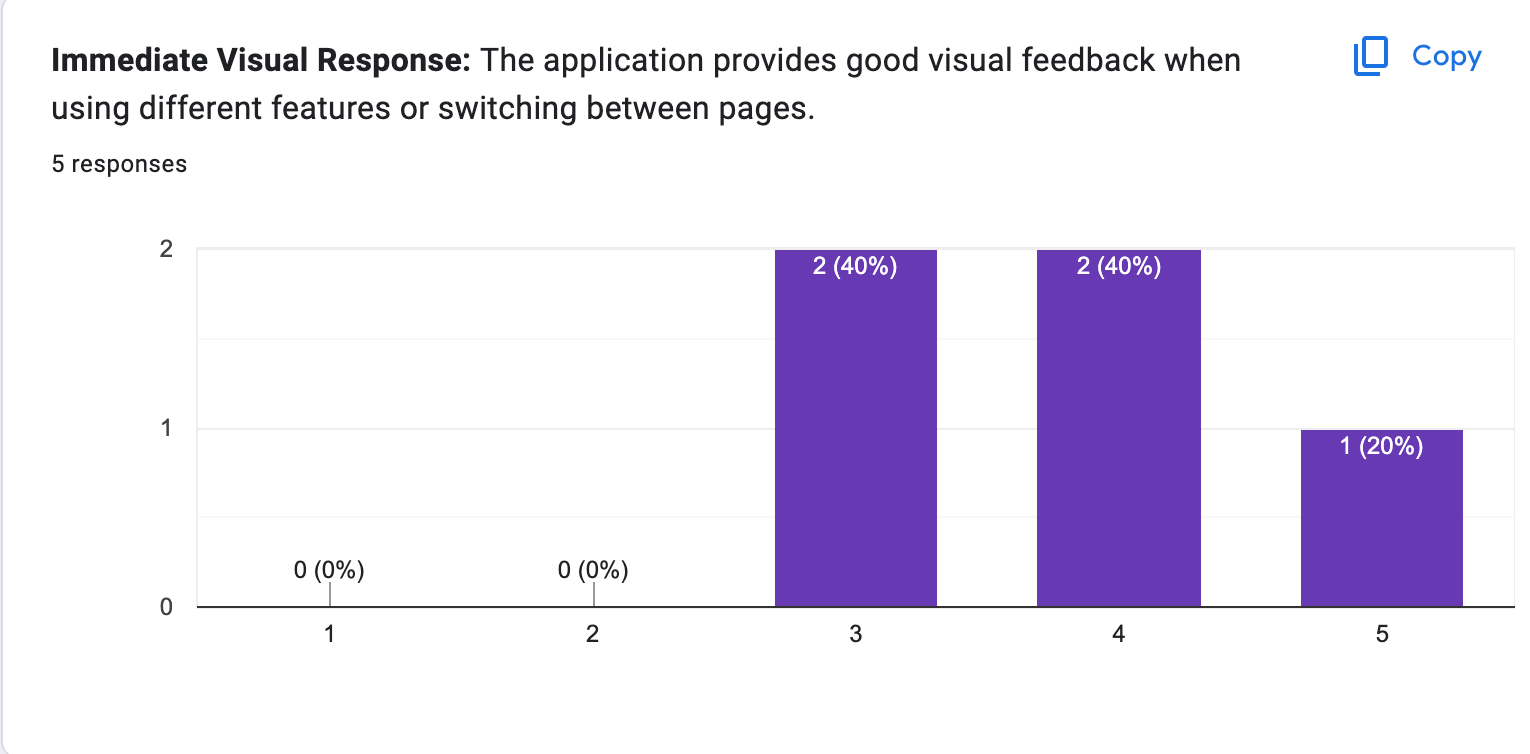
\includegraphics[scale=0.4]{Q1.png}
\item Appealing Colour Scheme: \textbf{4.8}\\
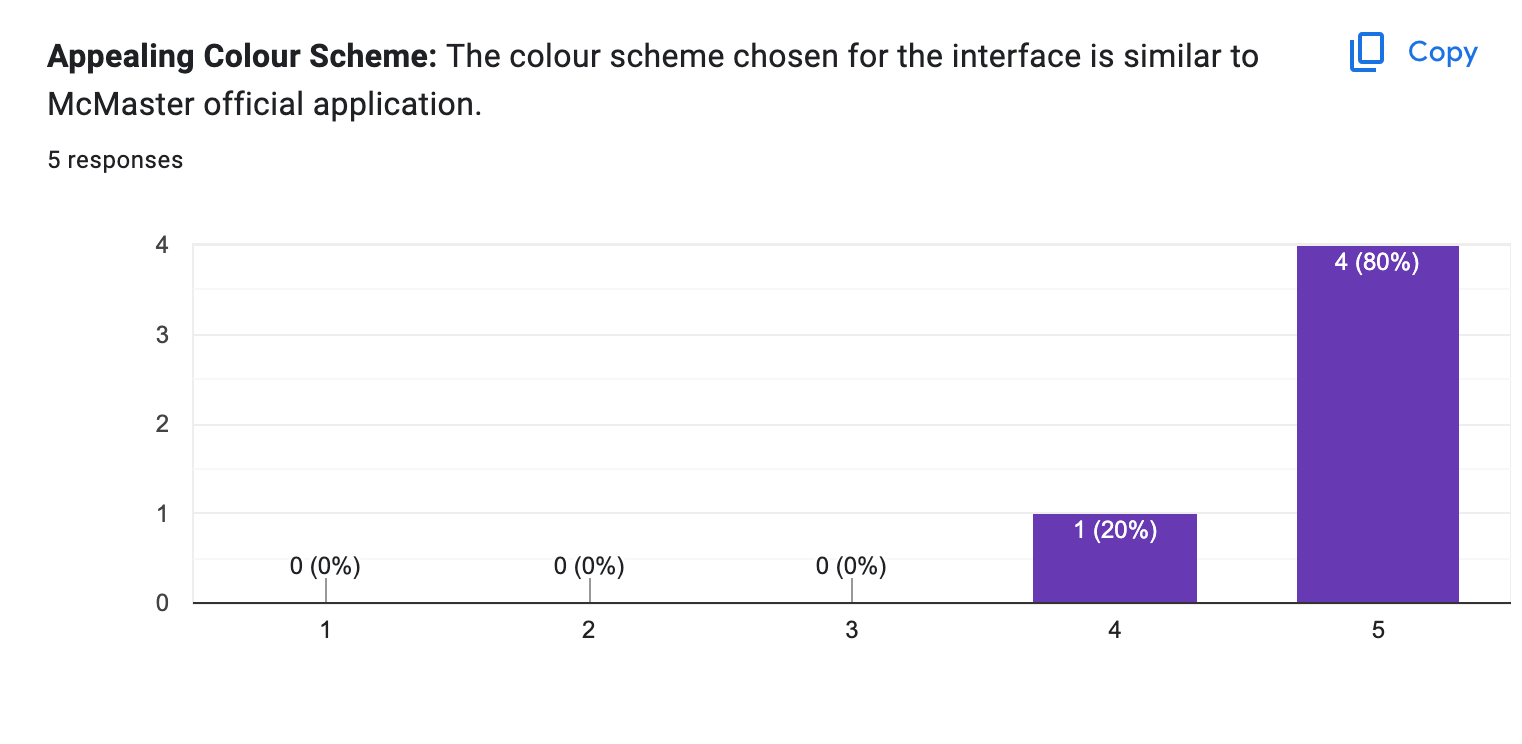
\includegraphics[scale=0.4]{Q2.png}
\item No Technical or Software-specific Language: \textbf{4}\\
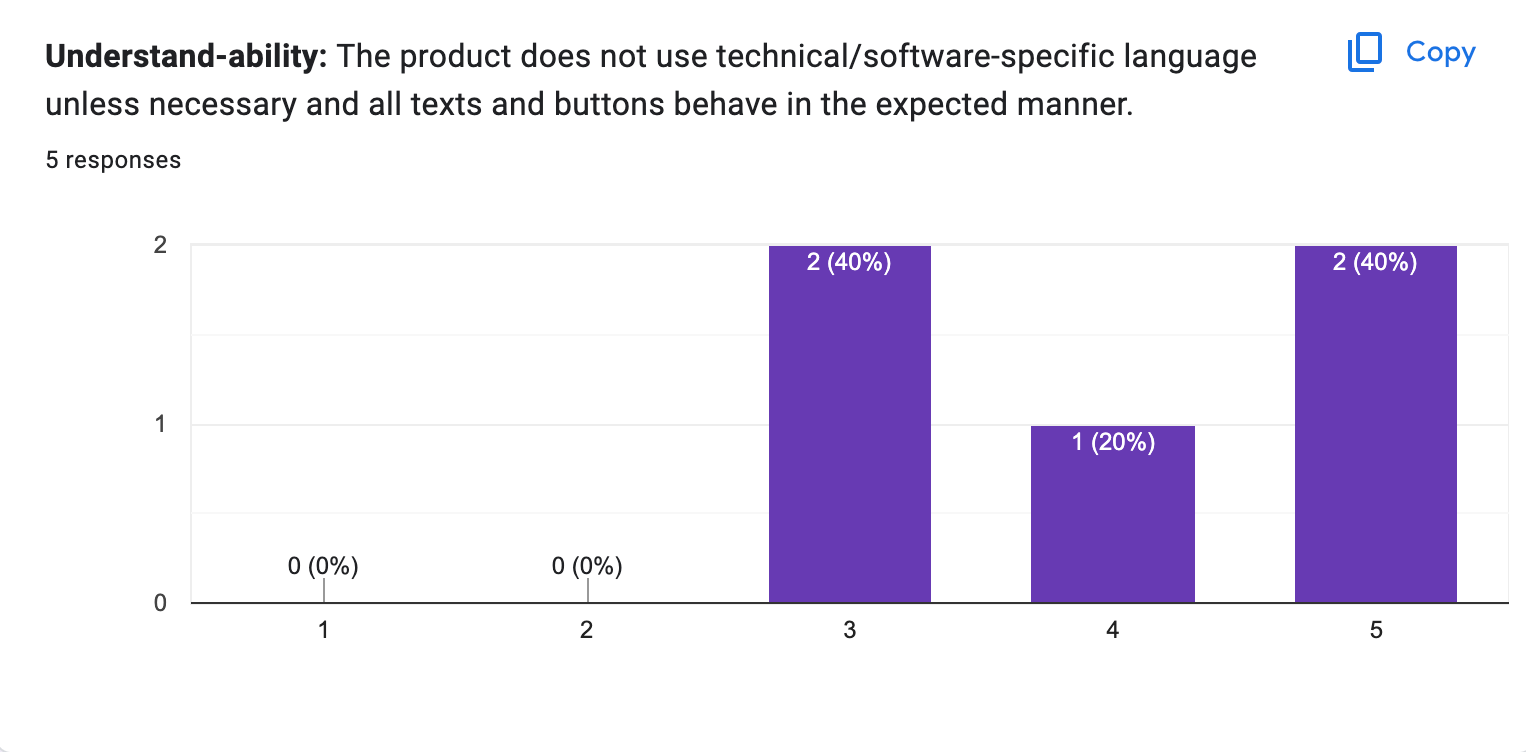
\includegraphics[scale=0.4]{Q3.png}
\item Common periods of usage: \textbf{3.2, \textcolor{red}{Fail}}\\
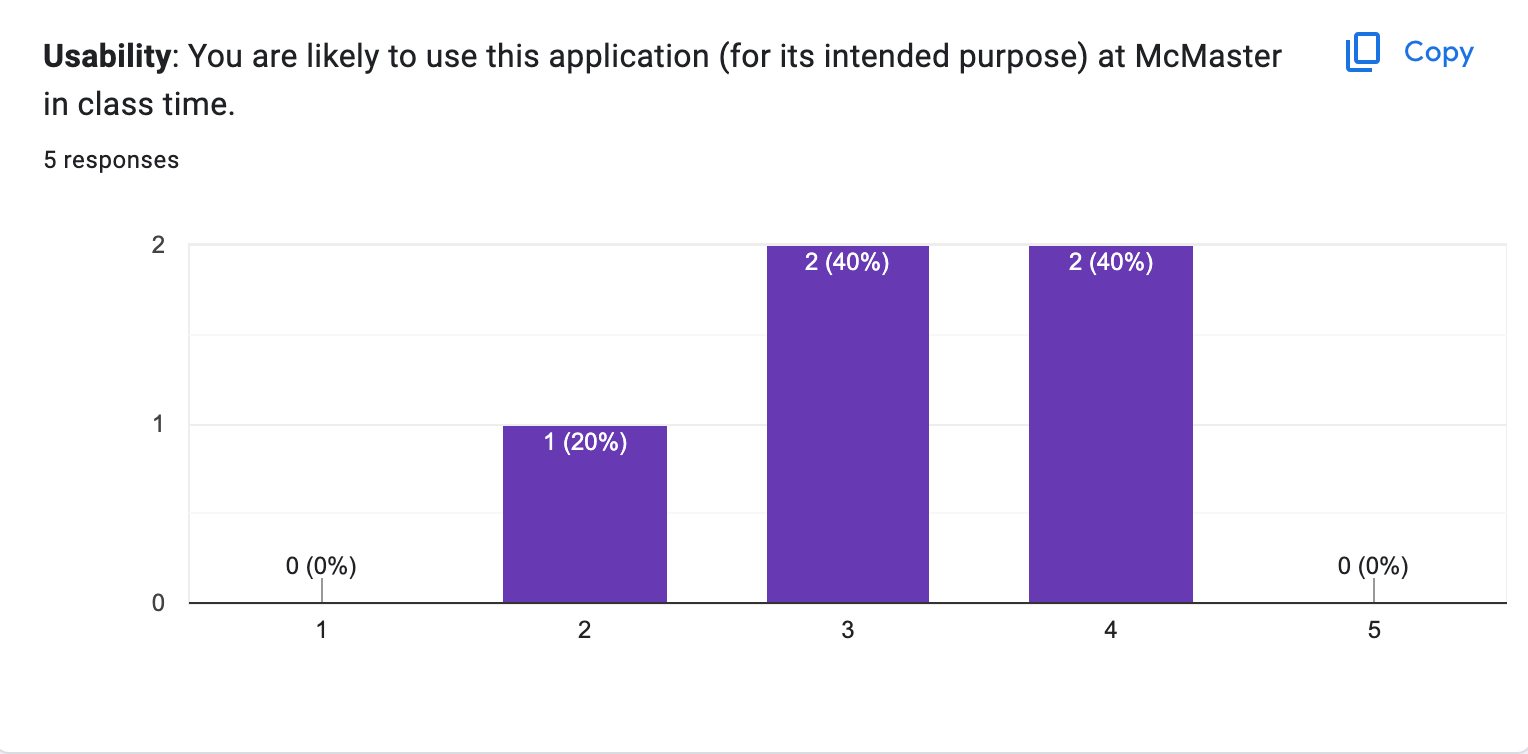
\includegraphics[scale=0.4]{Q4.png}
\item Cultural Friendliness: \textbf{4.8}\\
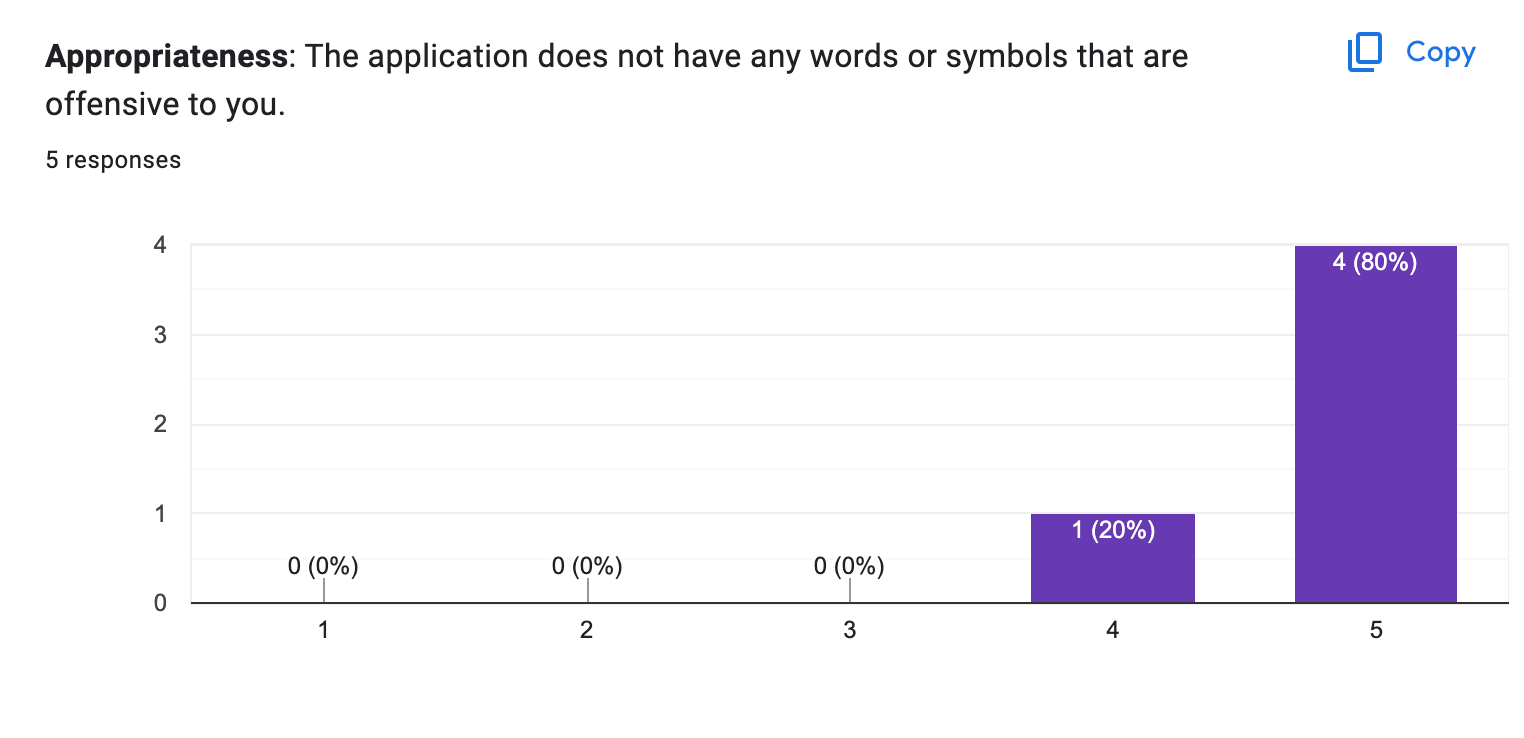
\includegraphics[scale=0.4]{Q5.png}
\end{itemize}
\subsection{Open-ended Question}
\begin{itemize}
\item Most difficult to use feature: \textbf{AR camera, pin, chatting}
\begin{enumerate}
\item The most difficult to use feature is probably the AR camera feature as it requires the user to use look through their phone camera while in buildings on campus. Additionally, it is also probably the most cool aspect of the app.
\item The lecture list isn't intuitive, there should be some calendar feature to show what days each lecture is running instead of just clicking on them, and maybe some more filters for building/location/course content.
\item The "pin" feature being hidden in the settings and the "AR Camera" not providing any feedback as to why we weren't seeing any were both confusing
\item The pinned/bookmarked events and lectures show up in a location (in settings) that is somewhat difficult to find. You also can't tap them to see more information about them on the pinned screen which is inconvenient.
\item Friend and chatting is unintuitive, don't know who I'm chatting with.
\end{enumerate}
\item Most likely to use feature: \textbf{Lecture/Event, AR camera}
\begin{enumerate}
\item Probably also the feature for looking up lecture events and times. This is useful as I can just open the app and view where specific lectures are located and choose to attend them or not.
\item I would use the AR camera feature to see interesting building history in between classes.
\item The feature that provided a schedule of all of the events was very nice
\item I could see the list of events at different locations being pretty useful, would be a good way to keep track of what's going on at Mac all in one place.
\item Events can be useful to see what is going on on campus and save events we want to go to
\end{enumerate}
\end{itemize}

\section{Load Test}\label{load}

This section covers results load testing of the backend server in details.
Testing was performed using Apache JMeter to simulate multiple concurrent users accessing the backend chat server. The objective of the test was to find the upper bound of concurrent users that can access the server without it crashing.
We discovered that it is rather difficult to crash a server being hosted on a cloud platform as there are several safeguards that prevent that.
Instead, we noticed that if too many connections are being made too quickly, then the server will just reject the most recently requested connections.

\newpage

We tested with various amounts of simulated users and observed how the server behaved. The results are plotted in the chart below.

\begin{table}[!htbp]
  \centering
  \begin{tabular}{|c|c|c|}
  \hline
  No. of Users & Server Rejected Connections? & Server Crashed? \\ \hline
  1 & No & No \\ \hline
  10 & No & No \\ \hline
  100 & No & No \\ \hline
  500 & No & No \\ \hline
  1000 & No & No \\ \hline
  5000 & Yes & No \\ \hline
  10000 & Yes & No \\ \hline
  \end{tabular}
  \caption{Load Testing Results}
\end{table}

We also observed analytics data from Microsoft Azure concerning the average response time of the server in relation to the number of requests.

\begin{figure}[!htbp]
  \centering
  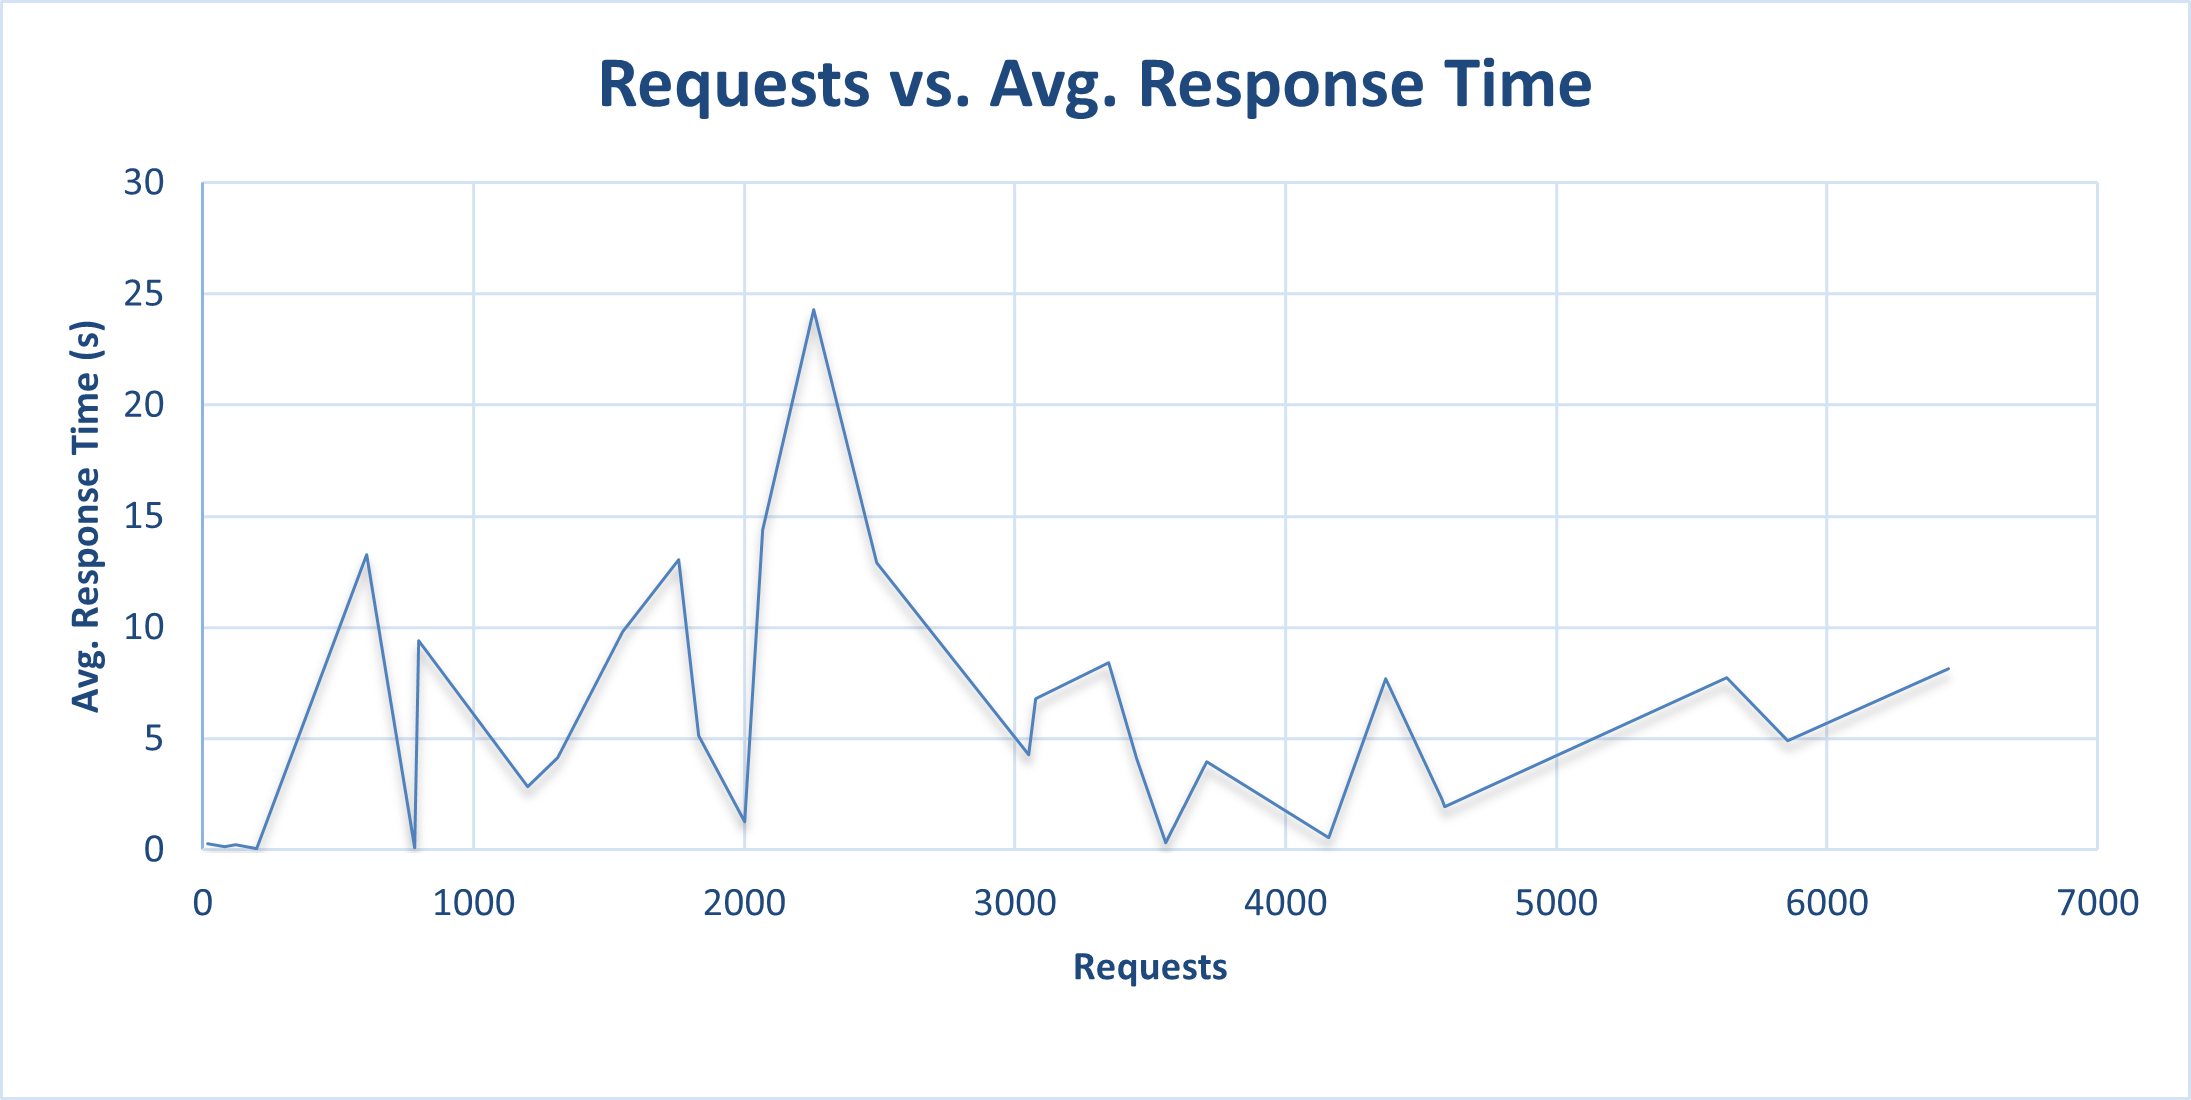
\includegraphics[width=\textwidth,keepaspectratio]{chart1.png}
  \caption{Requests vs. Response Time}
\end{figure}

There does not appear to be an observable trend. We believe this is because the test was limited by the amount of connections that could be made from one device.
Given a sufficient testing setup it should be possible to show a trend bewteen the amount of requests and the response time.

\section{Non dynamic Tests Result}\label{static}
The weekly meetings mentioned in the VnV Plan, such as the weekly code review and TA feedback sessions, will not be detailed in this section due to their frequency and the fact that many of the conclusions drawn in these meetings have already been integrated and addressed in other sections, particularly non-requirements. However, their meeting minutes are accessible on our GitHub repository for those interested in further details.
\begin{table}[H]
\caption{Nondynamic Test Result}
\begin{tabular}{|p{0.3\linewidth} | p{0.5\linewidth}| p{0.2\linewidth} |}
\hline
\multicolumn{1}{|l}{\bfseries Test Method} & \multicolumn{1}{|l|}{\bfseries Result} & \multicolumn{1}{l|}{\bfseries Related Test(s)}\\
\hline
Code Inspection for user data & 
\begin{itemize}
\item User permission: Pass, the application forces to user to sign a consent form when they register
\item Legitimate use of data: Pass, the supervisor points out that data are not used out of the application for any business purpose
\item Compliance: Pass, nothing violates McMaster privacy polices
\end{itemize} & NFRT-P3, NFRT-PRV1, NFRT-COM1 \\
\hline
Database Walkthrough & 
\begin{itemize}
\item Capacity: Pass, the free plan has a storage of 1GB data, which is enough for our users at this stage
\item Clean: Pass, Firebase Authentication support some clould functions to clean inactive users
\end{itemize}& NFRT-P15, NFRT-PRV2\\
\hline
Server \& Data Transmission Walkthrough & 
\begin{itemize}
\item Restart: Pass, the server is set to restart when it crashes
\item Encryption: pass, the data is encrypted in https
\end{itemize} & NFRT-P4, NFRT-P12 \\
\hline
Longevity Peer Evaluation & 
\begin{itemize}
\item Longevity: Pass, nothing in the code is dependent on the version of the device
\end{itemize} & NFRT-P17\\
\hline
\end{tabular}
\end{table}
\begin{table}[H]
\caption{Nondynamic Test Result Cont}
\begin{tabular}{|p{0.3\linewidth} | p{0.5\linewidth}| p{0.2\linewidth} |}
\hline
\multicolumn{1}{|l}{\bfseries Test Method} & \multicolumn{1}{|l|}{\bfseries Result} & \multicolumn{1}{l|}{\bfseries Related Test(s)}\\
\hline
Code Walkthrough with Primary Reviewers & 
\begin{itemize}
\item Issues: Pass, ia new building can be added like a game object in the project
\end{itemize} & NFTR-P16\\
\hline
GitHub Walkthrough with Reviewers & 
\begin{itemize}
\item Issues: Pass, issues are public to read and write in the repo
\item Instructions: Pass, there are instructions for developers and users in the repo
\end{itemize} & NFRT-UH2, NFRT-MS2\\
\hline
\end{tabular}
\end{table}

\section{Comparison to Existing Implementation}	

Not applicable to this project since there is no existing implementation.

\section{Unit Testing}
The following section outlines the results of unit testing. The process and test performed follow the \href{https://github.com/beatlepie/4G06CapstoneProjectTeam2/blob/main/docs/VnVPlan/VnVPlan.pdf}{VnV Plan}. \textcolor{red}{Due to the time constraint, we skipped the unit tests for Database and Authentication modules, but we will add unit tests for them in Revision 1.} Other than the two modules, all the tests pass, which indicates the low level modules of the system is implemented correctly and robustly.\\
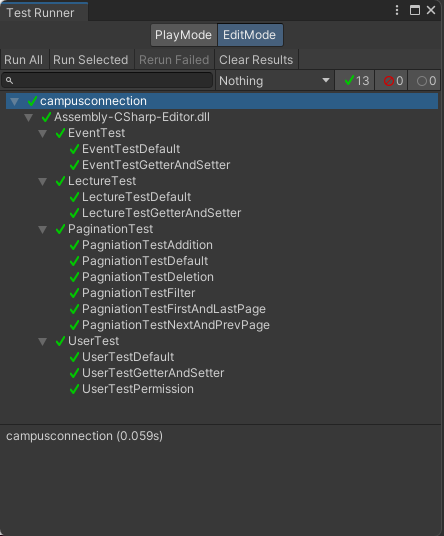
\includegraphics[scale=1]{Unit Test.png}
\subsection{User}
This section contains tests related to the module: User in module hierarchy.
\begin{enumerate}
\item \textbf{FRT-M1-1}

\textbf{Name:} Successful default user creation

\textbf{Initial State:} NA

\textbf{Input:} User identifier, email: unitTest@test.com
					
\textbf{Expected Output:} A user is successfully created with following attributes:
\begin{itemize}
\item email: unitTest@test.com
\item nickname: `'
\item photoURI: null
\item program: `'
\item level: 0
\item lectures: empty list of string
\item event: empty list of string
\item friends: empty list of string
\item friendInvitation: empty list of string
\end{itemize}

\textbf{Actual Output:} Same as expected output

\textbf{Result:} Pass

\item \textbf{FRT-M1-2}

\textbf{Name:} Successful new user creation

\textbf{Initial State:} NA

\textbf{Input:} User:
\begin{itemize}
\item email: unitTest@test.com
\item nickname: `Mr. Unit Test'
\item photoURI: http://example/com/photo.jpg
\item program: `software engineering'
\item level: 1
\item lectures: \{`Lecture 1', `Lecture 2'\}
\item event: \{`Event 1', `Event 2'\}
\item friends: \{`unitTest1@test.com', `unitTest2@test.com'\}
\item friendInvitation: \{`unitTest3@test.com'\}
\end{itemize}

\textbf{Expected Output:} A user is successfully created with attributes above

\textbf{Actual Output:} Same as expected output

\textbf{Result:} Pass
\end{enumerate}

\subsection{Event}
This section contains tests related to the module: Event in module hierarchy.
\begin{enumerate}
\item \textbf{FRT-M2-1}

\textbf{Name:} Successful default event creation

\textbf{Initial State:} NA

\textbf{Input:} Event identifier, name: unit test event

\textbf{Expected Output:} An event is successfully created with following attributes:
\begin{itemize}
\item name: unit test event
\item description: PLACEHOLDER
\item organizer: PLACEHOLDER
\item duration: DEFAULT\_DURATION
\item time: DEFAULT\_TIME
\item isPulbic: false
\item location: PLACEHOLDER
\end{itemize}

\textbf{Actual Output:} Same as expected output

\textbf{Result:} Pass

\item \textbf{FRT-M2-2}

\textbf{Name:} Successful new event creation

\textbf{Initial State:} NA

\textbf{Input:} Event:
\begin{itemize}
\item name: unit test event2
\item description: A unit test sample event
\item organizer: Team 2
\item duration: 30
\item time: 1708922625
\item isPulbic: true
\item location: Online
\end{itemize}
					
\textbf{Expected Output:} An event is successfully created with attributes above

\textbf{Actual Output:} Same as expected output

\textbf{Result:} Pass
\end{enumerate}

\subsection{Lecture}
This section contains tests related to the module: Lecture in module hierarchy.
\begin{enumerate}
\item \textbf{FRT-M3-1}

\textbf{Name:} Successful default lecture creation

\textbf{Initial State:} NA

\textbf{Input:} Lecture identifier, code: UNIT TEST3

\textbf{Expected Output:} A lecture is successfully created with following attributes:
\begin{itemize}
\item code: UNIT TEST3
\item name: PLACEHOLDER
\item instructor: PLACEHOLDER
\item time: PLACEHOLDER
\item location: PLACEHOLDER
\end{itemize}

\textbf{Actual Output:} Same as expected output

\textbf{Result:} Pass

\item \textbf{FRT-M3-2}

\textbf{Name:} Successful new lecture creation

\textbf{Initial State:} NA

\textbf{Input:} Lecture:
\begin{itemize}
\item code: UNIT TEST3
\item name: Unit test Lecture
\item instructor: Team 2
\item time: 12:30 - 13:30, Mon
\item location: Online
\end{itemize}

\textbf{Expected Output:} A lecture is successfully created with attributes above

\textbf{Actual Output:} Same as expected output

\textbf{Result:} Pass
\end{enumerate}

\subsection{Pagination}
This section contains tests related to the module: Pagination and Filter in module hierarchy.
\begin{enumerate}
\item \textbf{FRT-M4-1}

\textbf{Name:} Successful pagination creation

\textbf{Initial State:} NA

\textbf{Input:} List of Pizza:
\begin{itemize}
\item medium, cheese
\item large, veggie
\end{itemize}
pageCount = 2, filterBy and filterString are null

\textbf{Expected Output:} A pagination class is created with following attributes:
\begin{itemize}
\item entryList: List of pizza from input
\item filteredList: same as entryList
\item maxPage: 1
\item currentPage: 1
\item filterBy: null
\item filterString: null
\end{itemize}

\textbf{Actual Output:} Same as expected output

\textbf{Result:} Pass

\item \textbf{FRT-M4-2}

\textbf{Name:} Successful pagination creation with filter

\textbf{Initial State:} NA

\textbf{Input:} List of Pizza:
\begin{itemize}
\item medium, cheese
\item large, veggie
\item medium, pepperoni
\end{itemize}
pageCount = 2, filterBy = `size' and filterString = `medium'

\textbf{Expected Output:} A pagination class is created with following attributes:
\begin{itemize}
\item entryList: List of pizza from input
\item filteredList: List of medium pizza only
\item maxPage: 1
\item currentPage: 1
\item filterBy: `size'
\item filterString: `medium'
\end{itemize}

\textbf{Actual Output:} Same as expected output

\textbf{Result:} Pass

\item \textbf{FRT-M4-3}

\textbf{Name:} Successful pagination addition

\textbf{Initial State:} List of Pizza:
\begin{itemize}
\item medium, cheese
\item large, veggie
\end{itemize}
pageCount = 2, filterBy and filterString = null

\textbf{Input:} New pizza added to the list:
\begin{itemize}
\item medium, pepperoni
\end{itemize}

\textbf{Expected Output:} A pagination class is created with following attributes:
\begin{itemize}
\item entryList: List of all three pizza
\item filteredList: same as entryList
\item maxPage: 2
\item currentPage: 1
\item filterBy: null
\item filterString: null
\end{itemize}

\textbf{Actual Output:} Same as expected output

\textbf{Result:} Pass

\item \textbf{FRT-M4-4}

\textbf{Name:} Successful pagination deletion

\textbf{Initial State:} List of Pizza:
\begin{itemize}
\item medium, cheese
\item large, veggie
\item medium, pepperoni
\end{itemize}
pageCount = 2, filterBy and filterString = null
					
\textbf{Input:} New pizza to be deleted from the list:
\begin{itemize}
\item medium, pepperoni
\end{itemize}

\textbf{Expected Output:} A pagination class is created with following attributes:
\begin{itemize}
\item entryList: List of two pizza (cheese and veggie)
\item filteredList: same as entryList
\item maxPage: 1
\item currentPage: 1
\item filterBy: null
\item filterString: null
\end{itemize}

\textbf{Actual Output:} Same as expected output

\textbf{Result:} Pass

\item \textbf{FRT-M4-5}

\textbf{Name:} Next Page

\textbf{Initial State:} List of Pizza:
\begin{itemize}
\item medium, cheese
\item large, veggie
\item medium, pepperoni
\end{itemize}
pageCount = 2, filterBy and filterString = null
					
\textbf{Input:} Call next page method twice
					
\textbf{Expected Output:} Current page is updated only once:
\begin{itemize}
\item currentPage: 2
\end{itemize}

\textbf{Actual Output:} Same as expected output

\textbf{Result:} Pass

\item \textbf{FRT-M4-6}

\textbf{Name:} Previous Page

\textbf{Initial State:} List of Pizza:
\begin{itemize}
\item medium, cheese
\item large, veggie
\item medium, pepperoni
\end{itemize}
pageCount = 2, filterBy and filterString = null\\
Call next page method first
					
\textbf{Input:} Call previous page method twice
					
\textbf{Expected Output:} Current page is updated only once:
\begin{itemize}
\item currentPage: 1
\end{itemize}

\textbf{Actual Output:} Same as expected output

\textbf{Result:} Pass

\item \textbf{FRT-M4-7}

\textbf{Name:} Last Page

\textbf{Initial State:} List of Pizza:
\begin{itemize}
\item medium, cheese
\item large, veggie
\item medium, pepperoni
\end{itemize}
pageCount = 2, filterBy and filterString = null
					
\textbf{Input:} Call last page method
					
\textbf{Expected Output:} Current page is updated:
\begin{itemize}
\item currentPage: 2
\end{itemize}

\textbf{Actual Output:} Same as expected output

\textbf{Result:} Pass

\item \textbf{FRT-M4-8}

\textbf{Name:} First Page

\textbf{Initial State:} List of Pizza:
\begin{itemize}
\item medium, cheese
\item large, veggie
\item medium, pepperoni
\end{itemize}
pageCount = 2, filterBy and filterString = null\\
Call next page method first
					
\textbf{Input:} Call first page method
					
\textbf{Expected Output:} Current page is updated:
\begin{itemize}
\item currentPage: 1
\end{itemize} 

\textbf{Actual Output:} Same as expected output

\textbf{Result:} Pass
\end{enumerate}

\subsection{Authentication}
This section contains tests related to the module: Authentication in module hierarchy. \textcolor{red}{Due to the time constraint, we will finish unit tests for this module in Revision 1 following the same pattern}
\begin{enumerate}
\item \textbf{FRT-M5-1}

\textbf{Name:} Get current user email

\textbf{Initial State:} Current user email: `unitTest@test.com'
					
\textbf{Input:} NA
					
\textbf{Expected Output:} The email in the initial state

\textbf{Actual Output:} \textcolor{red}{TBD}

\textbf{Result:} \textcolor{red}{TBD}

\item \textbf{FRT-M5-2}

\textbf{Name:} Is email verified

\textbf{Initial State:} Current user is email verified: true
					
\textbf{Input:} NA
					
\textbf{Expected Output:} The boolean value in initial state 

\textbf{Actual Output:} \textcolor{red}{TBD}

\textbf{Result:} \textcolor{red}{TBD}

\item \textbf{FRT-M5-3}

\textbf{Name:} Verify email

\textbf{Initial State:} Current user email: `unitTest@test.com'
					
\textbf{Input:} Call verify email method
					
\textbf{Expected Output:} An email is sent to the email address to verify the email

\textbf{Actual Output:} \textcolor{red}{TBD}

\textbf{Result:} \textcolor{red}{TBD}
\end{enumerate}

\subsection{Database}
This section contains tests related to the module: Database in module hierarchy. \textcolor{red}{Due to the time constraint, we will finish unit tests for this module in Revision 1 following the same pattern}
\begin{enumerate}
\item \textbf{FRT-M6-1}

\textbf{Name:} Get value

\textbf{Initial State:} NA
					
\textbf{Input:} A valid path to a test node: `/events/public/EXPO/name'
					
\textbf{Expected Output:} The corresponding value of the node: EXPO

\textbf{Actual Output:} \textcolor{red}{TBD}

\textbf{Result:} \textcolor{red}{TBD}

\item \textbf{FRT-M6-2}

\textbf{Name:} Set value

\textbf{Initial State:} NA
					
\textbf{Input:} A valid path to a test node and a new value: 
\begin{itemize}
\item path: `/events/public/EXPO/description'
\item value: `EXPO, yes!'
\end{itemize}

\textbf{Expected Output:} The corresponding value changes to the new value

\textbf{Actual Output:} \textcolor{red}{TBD}

\textbf{Result:} \textcolor{red}{TBD}

\item \textbf{FRT-M6-3}

\textbf{Name:} Delete data

\textbf{Initial State:} NA
					
\textbf{Input:} A valid path to a test node : `/events/public/EXPO'

\textbf{Expected Output:} The corresponding event is removed

\textbf{Actual Output:} \textcolor{red}{TBD}

\textbf{Result:} \textcolor{red}{TBD}
\end{enumerate}

\section{Changes Due to Testing}
\subsection{Changes due to Rev 0 demo feedback}
In Revision 0 of the demonstration, our instructor, Dr. Smith, pointed out that certain features, such as access control and the event list page, had not yet been implemented. These aspects were accorded higher priority in the development plan and have been successfully completed.

\subsection{Changes due to supervisor's feedback}
During the weekly meeting, our supervisor, Dr. Yuan, emphasized the necessity of reducing the sample size for the usability survey at this stage, which had previously been set at 50. Additionally, Dr. Yuan suggested incorporating tasks into the survey to facilitate thorough testing of the application by users. Consequently, the team collectively decided to integrate tasks and open-ended questions into the usability survey. This adjustment aims to gather more insightful feedback, discerning which aspects users like most and pinpointing features requiring improvement from a usability perspective.
\subsection{Changes due to usability test result}
The only test fails is the ``Common periods of usage'' rating question. It has come to light that survey participants express a preference for utilizing the application after school so that they won't miss any events happen in the evening. This observation is directly linked to maintenance requirement MS-M1. The team will change that major update time in that requirement to be summer break or weekend midnight to affect fewer users.\\
The absence of instructions for the AR camera has been repeatedly highlighted in the feedback. Consequently, the team will resolve this issue by adding instructions when user clicks on the help button. \\
Participants have noted that saved lectures and events are not readily accessible, as they are currently hidden within the settings. In response to this feedback, the team will create a link to the saved lectures and events page directly from the list pages. \\
Each of the aforementioned changes will be documented as a separate issue in the GitHub repo for future discussion.\\
\subsection{Changes due to load test result}
The load test in section \ref{load} shows that NFRT-P16 passes without any issues -- with fewer than 1000 users connecting to the application, the server handles the load effectively, as indicated by the nearly negligible response time observed in the figure. However, it is crucial to note that upon scaling up to accommodate approximately 40,000 concurrent requests after Revision 1, the server begins to reject connections and getting a significant increase in response time.Therefore, this is a good warning for the team regarding the need to scale the server infrastructure adequately to support a larger user base.
\subsection{Changes due to failing tests}
NFRT-P10 fails due to a change of the scope. The team will update SRS and VnV Plan so that internet connection lost warning is no longer a requirement.
\subsection{Changes due to user enumeration vulnerability}
\textcolor{red}{\textbf{If granted additional time, the team will implement the following changes:}}

User enumeration occurs when a malicious actor utilizes brute-force techniques to guess or confirm valid users within the system. In our application, this vulnerability can occur during the login process, where attackers can determine the validity of an email by analyzing error messages. Therefore,  the team proposes implementing a more generic error message during login attempts (FRT-UA4). Additionally,, a new test should be added to verify unsuccessful login attempts using an email not registered in the system.

On the other hand, the password recovery page effectively prevents this type of attack by only checking for email format without revealing whether the email exists in the system. 

Moreover, there are concerns regarding attackers exploiting server response times to detect user existence but that does not seem to be a problem with our application as Firebase's real-time database responds to valid and invalid login attempts with indistinguishable time differences.

Considering the project's scope and potential visibility (most of our customers will be students and department staff), frequent enumeration attacks are unlikely. Nevertheless, the aforementioned measures should sufficiently safeguard against such attacks.

\section{Automated Testing}
The tests are run from local machine as there were difficulties in implementing GitHub Action for it.
When attempting to setup the automated tests, there were issues due to how Vuforia was not a package that could be imported automatically.
This caused problems as the program failed to build automatically. The package was too big to be included in the repository, and Large File Storage had limits.
Due to the above reason, automated tests could not be performed through GitHub Actions, they could be run on local.
Parts of the below documentation is based on what was planned, and what is planned for phase 2 of the development.

\subsection{Testing Instruments}

The tests were performed using Unity Testing Framework, NUnit made for Unity.
The test files are located in multiple files with the respective names of the modules they are testing under Assets/Editor.
OpenCover was planned for coverage testing and will produce a report into XML file.
These results are visible after the automated tests are completed.
The CI with GitHub Actions will be completed in phase 2.

\subsection{Linters}

Linters were added into CI using Super-linter. This is an open source linter maintained and used by many people, which shows its reliability.
The linter only checks the new contents in the repository, making it efficient and concise. 
The code linter has been active and we have fixed issues brought up by the test results such as duplicate code and formatting issues.
The results of linters are visible under the GitHub Actions tab.

\section{Trace to Requirements}
See Traceability tables between Test Cases and Requirements in \href{https://github.com/beatlepie/4G06CapstoneProjectTeam2/blob/main/docs/VnVPlan/VnVPlan.pdf}{VnV Plan}
\section{Trace to Modules}		
See Traceability tables between Test Cases and Modules in \href{https://github.com/beatlepie/4G06CapstoneProjectTeam2/blob/main/docs/VnVPlan/VnVPlan.pdf}{VnV Plan}, notice that M5 and M6 are not completed yet in this iteration.

\section{Code Coverage Metrics}
The code coverage report can be seen in the \href{https://github.com/beatlepie/4G06CapstoneProjectTeam2/blob/main/docs/VnVReport/Report.zip}{zip folder}.
The report contains all files in the project, which some are libraries or Unity files.
The relevant code coverage data is shown in the table below.

Due to the time constraints, authentication and database tests were pushed to phase 2.
The testing files are located in \href{https://github.com/beatlepie/4G06CapstoneProjectTeam2/tree/feat-testing-tests/src/CampusConnections/Assets/Editor}{folder}.

\begin{table}[h]
  \begin{tabular}{lll}
  \hline
  Module                   & Code Coverage & Test Module    \\
  \hline
  User                     & 100\%         & UserTest       \\
  Pagination               & 95.8\%        & PaginationTest \\
  Event                    & 100\%        & EventTest      \\
  Lecture                  & 100\%        & LectureTest    \\
  \hline
  \end{tabular}
  \end{table}

\newpage{}
\section*{Appendix}
\subsection{Symbolic Parameters}
Check the Symbolic Parameter Table in \href{https://github.com/beatlepie/4G06CapstoneProjectTeam2/blob/main/docs/VnVPlan/VnVPlan.pdf}{VnV Plan} for more details.

The following table only contains symbols that appear only in the report
\begin{table}[H]
\caption{\bf Symbolic Parameter Table}
\begin{tabular}{|p{0.4\linewidth} | p{0.3\linewidth}| p{0.3\linewidth} |}
\hline
\multicolumn{1}{|l}{\bfseries Symbolic Parameter} & \multicolumn{1}{|l|}{\bfseries Description} & \multicolumn{1}{l|}{\bfseries Value}\\
\hline
Femail & The friend email, an email that exists in the application database, usually used with target email to test user communication & Value depends on the test it belongs to\\
\hline
Temail & The target email, an email that exists in the application database, usually used with friend email to test user communication & Value depends on the test it belongs to\\
\hline
\end{tabular}
\end{table}

\subsection{Reflection}
The information in this section will be used to evaluate the team members on the
graduate attribute of Reflection.  Please answer the following question:

\begin{enumerate}
  \item In what ways was the Verification and Validation (VnV) Plan different
  from the activities that were actually conducted for VnV?  If there were
  differences, what changes required the modification in the plan?  Why did
  these changes occur?  Would you be able to anticipate these changes in future
  projects?  If there weren't any differences, how was your team able to clearly
  predict a feasible amount of effort and the right tasks needed to build the
  evidence that demonstrates the required quality?  (It is expected that most
  teams will have had to deviate from their original VnV Plan.)
\end{enumerate}

The execution of our testing plan was very different from how we initially envisioned in our VnV Plan. The VnV plan was written before any implementation had been done.
This resulted in us making several assumptions about how the final product would work. Of course, as our project evolved, many of our assumptions would need to be changed.\\

One of the main ways our actual VnV testing effort varied was the scope of what was tested. Due to time constraints, some of our planned features needed to be cut.
This resulted in some proposed test cases no longer being applicable. While it is natural for requirements and scope to change throughout a project's life, the invalidation of these tests
could potentially have been mitigated by creating the VnV Plan when the structure of the project is more concrete. In future VnV planning, we would either do our VnV planning after completing some of the
implementation, or by iterating on the previous VnV by making amendments and revisions.\\

Another thing that impacted our VnV testing effort was our level of familiarity with the testing tools available and how they interacted with our technology stack.
For example, we initially wanted to test our database-facing front-end code using the Unity Test Framework (UTF). Due to our lack of experience with UTF and Firebase, we assumed that
it would be possible to test Firebase code using UTF. This ended up not being the case and the tests that were planned were scrapped or pushed to our feature waiting list. In future VnV planning, we would
put more effort into learning the tools and technology needed to test our project before coming up with test plans.\\

Comparing how our testing efforts went with how we planned them taught us that it is best to be conservative with the scope of features as some development time must
be allocated to testing those features. We also learned to value iterative improvement by keeping the documentation ``alive'' with revisions along with the project.
Lastly, we gained experience with a wide variety of testing tools and techniques that will be valuable in future VnV planning and execution.

\end{document}